% todo - biologicke pojmy (ale nie vela) definovat hlavne informaticky problem
% obrazok zarovnania - sekvencie, okno, anotacie
% menej slovies - doplnit pri prednasani

% ak budem mať CRF tak porovnanie CRF a HMM - pozret rydzikovu prezentaciu

% Motivacia, ine vysledky
% Ohurit komisiu
% Urobili vela prace, Nebolo to lahke

% popisat tranzitivitu
% popisat referencne modely

\documentclass[xcolor=dvipsnames, compress, 12pt]{beamer}
\usepackage[utf8]{inputenc}
\usepackage[slovak]{babel}
\usepackage{lmodern}
\usepackage[T1]{fontenc}
\usepackage{amsfonts}
\usepackage{amssymb}
\usepackage{amsthm}
\usepackage{amsmath}
\usepackage{epsfig}
\usepackage{wrapfig}
\usepackage{caption}
\usepackage{subcaption}
\usepackage{url}
\usepackage{hyperref}
\usepackage{multicol}
\usepackage{fancyvrb}
\usepackage{tabu}
\usepackage{multirow}
\usepackage{booktabs}
\usepackage{regexpatch}
\makeatletter
% Change the `-` delimiter to an active character
\xpatchparametertext\@@@cmidrule{-}{\cA-}{}{}
\xpatchparametertext\@cline{-}{\cA-}{}{}
\makeatother

\usecolortheme[named=Green]{structure}
\usetheme{Madrid}
\setbeamertemplate{navigation symbols}{}
\usebackgroundtemplate{
\includegraphics[width=\paperwidth, height=\paperheight]{images/bg.png}}
\setbeamercovered{transparent}

% \setbeamertemplate{footline}[frame number]
% \setbeamertemplate{items}[ball]
% \setbeamertemplate{blocks}[rounded][shadow=true]
% \useoutertheme{umbcfootline}

% \AtBeginSection[]{
% \frame<beamer>{

%     \ifpdf
%       \pdfbookmark[0]{Contents}{toc}
%     \fi
%     \frametitle{Obsah}
%     \setcounter{tocdepth}{2}
%     \tableofcontents[currentsection,subsections,hideothersubsections]

% }
% }

% Show frame number in footbar
\setbeamertemplate{footline}%{miniframes theme}
  {%
    \begin{beamercolorbox}[colsep=1.5pt]{upper separation line foot}
    \end{beamercolorbox}
    \begin{beamercolorbox}[ht=2.5ex,dp=1.125ex,%
      leftskip=.3cm,rightskip=.3cm plus1fil]{author in head/foot}%
      \leavevmode{\usebeamerfont{author in head/foot}\insertshortauthor}%
      \hfill%
      {\usebeamerfont{institute in head/foot}\usebeamercolor[fg]{institute in head/foot}\insertshortinstitute}%
    \end{beamercolorbox}%
    \begin{beamercolorbox}[ht=2.5ex,dp=1.125ex,%
      leftskip=.3cm,rightskip=.3cm plus1fil]{title in head/foot}%
      {\usebeamerfont{title in head/foot}\insertshorttitle} \hfill     \insertframenumber
      % /\inserttotalframenumber %
    \end{beamercolorbox}%
    \begin{beamercolorbox}[colsep=1.5pt]{lower separation line foot}
    \end{beamercolorbox}
  }

% items enclosed in square brackets are optional; explanation below
\title{Zarovnávanie sekvencií s~použitím metód klasifikácie}
\subtitle{
\vspace{0.5cm}
\small Diplomová práca
}
\author[Michal Hozza]{\small Bc. Michal Hozza \\ \vspace{1cm} \footnotesize \textbf{Vedúci práce:} Mgr. Tomáš Vinař, PhD. \\ \textbf{Konzultant:} Mgr. Michal Nánási\\ \vspace{.5cm}}
\institute[FMFI UK \insertshortdate]{
  Fakulta matematiky, fyziky a informatiky,
  Univerzita Komenského, Bratislava\\
}
\date[\the\year]{\footnotesize \today}

\newcommand{\lenitem}[2][.6\linewidth]{\parbox[t]{#1}{\strut #2\strut}}

\newtheorem{vt}{Veta}[section]
\newtheorem{lema}[vt]{Lema}
\theoremstyle{definition}
\newtheorem{df}[vt]{Definícia}

\begin{document}

%--- the titlepage frame -------------------------%
\begin{frame}[plain]
  \titlepage
\end{frame}

%--- the presentation begins here ----------------%

\begin{frame}{Obsah}
  \transdissolve[duration=0.1]
  % \begin{multicols}{2}
  \tableofcontents
  % \end{multicols}
\end{frame}


\section{Úvod}

\subsection{Cieľ}
\begin{frame}{Cieľ}
  % \transdissolve
  \begin{itemize}
  \item cieľom práce je vytvoriť nové metódy na korekciu zarovnaní biologických sekvencií na základe prídavnej informácie
  \item integrácia tejto informácie bude zabezpečená pomocou techník využívaných na klasifikáciu v~strojovom učení
  \end{itemize}
\end{frame}

\subsection{Zarovnávanie sekvencií}
\begin{frame}[fragile]{Zarovnávanie sekvencií}
  \begin{itemize}
      \item jedným zo základných bioinformatických problémov
      \item identifikuje časti sekvencie, ktoré vznikli z~toho istého predka (zarovnané bázy), inzercie a delécie v~priebehu evolúcie (medzery v~zarovnaní)
  \end{itemize}
\pause
\begin{df}[Globálne zarovnanie]
Vstupom sú dve sekvencie $X = x_1x_2\dots x_n$ a $Y = y_1y_2\dots y_m$
Výstupom je zarovnanie celých sekvencií $X$ a $Y$.
\end{df}
\pause
Príklad:
      \begin{verbatim}
  GTGGACCGTT------CCTTCCGGCAATCACGAGAAAAGCCACGT
  GTCGACCGTTTCAGTGACTTGAAGCAATCAGG---AACACCACCT
      \end{verbatim}
\end{frame}

\begin{frame}{Skryté Markovovské modely}
  \begin{itemize}
    \item pravdepodobnostný model inšpirovaný konečnými automatmi
    \item pozostáva z 3 distribúcií
    \begin{itemize}
        \item distribúcia začiatočných stavov ($\pi_i$)
        \item distribúcia prechodov ($a_{i,j}$)
        \item distribúcia emisií ($e_{i,x}$)
    \end{itemize}
    \pause
    \item pravdepodobnosť, že model vygeneruje sekvenciu $x$ dĺžky $n$ s~anotáciou $s$ je súčin pravdepodobností prechodov a emisií.
    $$P(X=x | S=s) = \pi_{s_1}\left(\prod_{i=1}^{n-1} e_{s_i,x_i} a_{s_i,s_{i+1}}\right)e_{s_n,x_n}$$
    \cite{skripta, durbin}

  \end{itemize}
\end{frame}

\begin{frame}{Zarovnávanie sekvencií pomocou pHMM}
  \mbox{}\hfill\raisebox{-\height}[0pt][0pt]{
   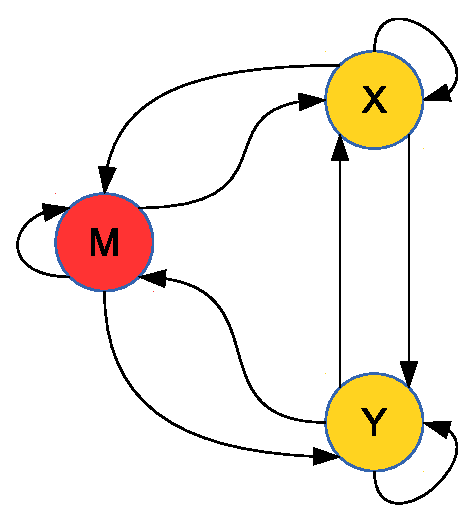
\includegraphics[width=.30\textwidth]{images/simple_model}
   }
  \vspace*{-\baselineskip}

  \begin{itemize}
    \item \lenitem{3 stavový pHMM}
    \begin{itemize}
      \item \lenitem{Match -- emituje dvojice:\\ $AA, AC, AG,\dots, TT$}
      \item \lenitem{Insert X, Insert Y -- emitujú jednotlivé bázy $A,C,G,T$}
    \end{itemize}
    \item \lenitem{prechodové a emisné pravdepodobnosti sa trénujú pomocou frekvenčnej tabuľky}
    \item najpravdepodobnejšie zarovnanie nájdeme pomocou Viterbiho algoritmu
  \end{itemize}
\end{frame}

% \begin{frame}{Inverzné zarovnanie}
%   \begin{df}[Problém inverzného zarovnania]
%   Vstupom sú dve sekvencie $X$, $Y$ a ich zarovnanie $Z$.
%   Výstupom sú parametre, podľa ktorých je toto zarovnanie optimálne.
%   \end{df}

%   \begin{itemize}
%     \item pod parametrami rozumieme skórovací systém -- napr. skórovaciu maticu alebo skrytý markvovský model
%   \end{itemize}
% \end{frame}

% \section{Modely a Existujúce riešenia}
% \subsection{Modely}
% \begin{frame}{Modely}
% Generatívny:
% \begin{itemize}
% \item sa snaží modelovať proces, ktorý generuje dáta ako pravdepodobnosť $P(X,Y,Z)$
% \item rozložíme ju pomocou nezávislých predpokladov na procese $\longrightarrow$ obmedzujúce
% \end{itemize}
% \pause
% Diskriminačný
% \begin{itemize}
% \item priamo odhaduje $P(Z|X,Y)$ alebo prislúchajúcu diskriminačnú funkciu, a preto sa zamerá na podstatnú časť problému odhadu
% \item Nepotrebuje nezávislosť $\longrightarrow$ silnejšie
% \end{itemize}
% \end{frame}

% % ToDo - lepsie popisat existujuce modely
% \subsection{Príbuzné témy}
% \begin{frame}{Príbuzné témy (existujúce riešenia)}
%   \begin{itemize}
%     \item Problém inverzného zarovnania
%     \pause
%     \item Support vector training of protein alignment models
%     \begin{itemize}
%       \item Support Vector Machine (SVM)
%       \item Umožňuje trénovať pomocou rôznych účelových funkcií
%     \end{itemize}
%     \pause
%     \item Contralign: Discriminative training for protein sequence alignment.
%     \begin{itemize}
%       \item Conditional Random Fields (CRF)
%       \item Neumožnuje trénovať pomocou rôznych účových funkcií
%     \end{itemize}
%   \end{itemize}
% \end{frame}

% \section{Naše riešenia}
% \subsection{Odlišnosti nášho riešenia}
% \begin{frame}{Odlišnosti nášho riešenia}
%   \begin{itemize}
%     \item Korekcia existujúcich zarovnaní
%     \begin{itemize}
%       \item Použitie súbežne s~existujúcimi zarovnávačmi
%     \end{itemize}
%     \pause
%     \item Rôzne modely využitia klasifikátora
%     \pause
%     \item Rôzne metódy trénovania
%     \pause
%     \item Možnosť učenia bez učiteľa
%     \pause
%     \item Iný klasifikátor
%     \begin{itemize}
%       \item možno porovnanie viac rôznych klasifikátorov
%       \item pípadne abstrakcia od klasifikátora
%     \end{itemize}
%   \end{itemize}
% \end{frame}


% \subsection{Simulátor}
% \begin{frame}{Simulátor}
%   \begin{itemize}
%     \item Model určený na prvotné experimenty
%     \item Program simuluje evolúciu
%     \begin{itemize}
%       \item Generovanie dvojice postupností so správnym zarovnaním
%       \item Generovanie dodatočej informácie
%       \item Simulácia mutácie a delécie
%     \end{itemize}
%   \end{itemize}
% \end{frame}

%ToDo: Obrázok
\section{Existujúce riešenia}
\begin{frame}{Existujúce metódy zarovnávania sekvencií s dodatočnou informáciou}
  \begin{df}[Problém inverzného zarovnania]
  Vstupom sú dve sekvencie $X$, $Y$ a ich zarovnanie $Z$.
  Výstupom sú parametre, podľa ktorých je toto zarovnanie optimálne.
  \end{df}
  \pause
  \begin{itemize}
    \item doterajšie publikácie boli o zarovnávaní proteínových sekvencií
    \item doterajší výskum sa zaoberal havne riešením problému IZ
    \item v \cite{svmTrainingProteinsAlignment} využili SVM na nájdenie parametrov a použili anotáciu o štruktúre sekvencií
    \item podobný prístup zvolili v \cite{contralign}, kde na nájdenie parametrov využili CRF
    \pause
    \item obe riešenia ťažia z výhod diskriminatívneho učenia, kde hľadáme $P(Z|W)$ (namiesto $P(Z,W)$, ktoré hľadáme pri generatívnych modeloch)
  \end{itemize}
\end{frame}


\section{Naše riešenie}
\begin{frame}{Naše riešenie}
  \begin{itemize}
    \item zarovnávanie s dodatočnou informáciou
    \item dodatočnú informáciu sme zakomponovali pomocou klasifikátorov
    \begin{itemize}
      \item klasifikátory na základe lokálnej informácie rozhodujú, či dané pozície majú byť zarovnané k sebe
      \item natrénujeme ich na existujúcich zarovnaniach
    \end{itemize}
    \item klasifikátory sme zakomponovali do pHMM pre zarovnávanie
  \end{itemize}
\end{frame}

\begin{frame}{Naše riešenie -- odlišnosti}
  \begin{itemize}
    \item zaoberáme sa DNA sekvenciami, nie proteínmi
    \item nemáme k~dispozícii sekundárnu štruktúru, ale iný typ anotácií
    \item naše modely sú kombináciou generatívneho a diskriminačného prístupu
    \item naše modely sú založené na pHMM
    \item používame dva rôzne klasifikátory
    \item architektúry našich modelov abstrahujú od klasifikátora
    \item ako klasifikátor sme použili \emph{náhodný les (angl. Random forest)} \cite{randomForestPaper}
  \end{itemize}
\end{frame}

\subsection{Klasifikácia na základe lokálnej informácie}

\begin{frame}{Klasifikácia na základe lokálnej informácie}
\begin{itemize}
  \item anotácie sme zakomponovali pomocou dvoch typov klasifikátorov
  \begin{enumerate}
    \item Match -- rozhoduje či dané pozície majú byť zarovnané k~sebe
    \item Indel -- rozhoduje či daná pozícia má byť zarovnaná k medzere
  \end{enumerate}
  \item výstup $\in \left<0,1\right>$ -- istota klasifikátora, že dané dve pozície majú byť zarovnané k~sebe (v~insert stave, že daná pozícia má  byť zarovnaná k~medzere)
  \item atribúty sú okná veľkosti $w$
\end{itemize}
\end{frame}

\begin{frame}{Okno pre klasifikátor}
\begin{figure}[h]
        \centering
        \begin{subfigure}[b]{0.35\textwidth}
                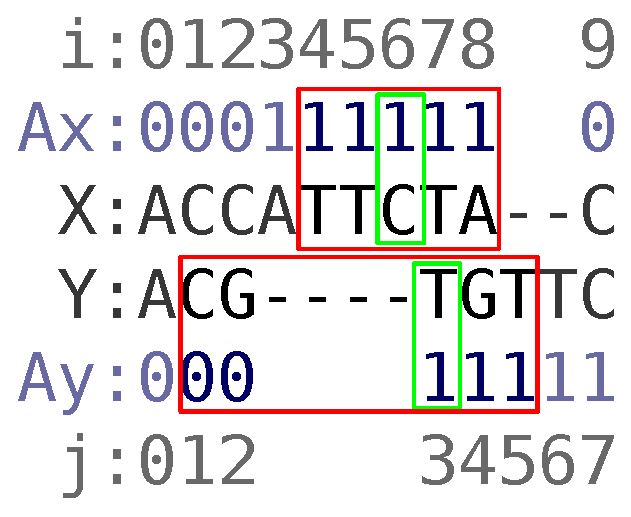
\includegraphics[width=\textwidth]{images/window_m}
                \caption{Match klasifikátor}
                \label{fig:window-m}
        \end{subfigure}%
        \qquad\qquad %add desired spacing between images, e. g. ~, \quad, \qquad etc.
          %(or a blank line to force the subfigure onto a new line)
        \begin{subfigure}[b]{0.35\textwidth}
                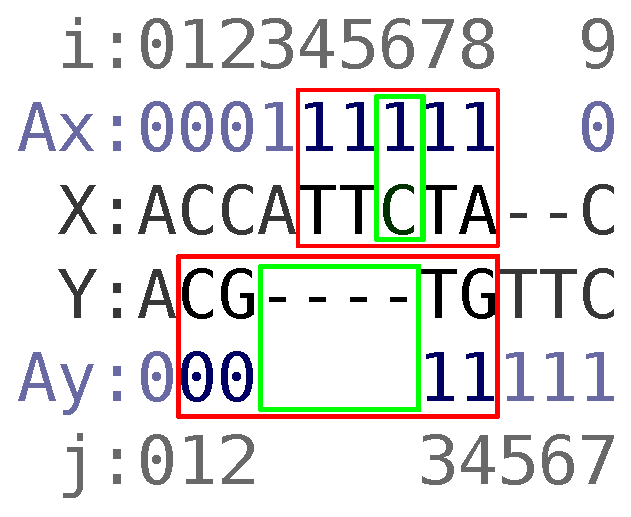
\includegraphics[width=\textwidth]{images/window_i}
                \caption{InDel klasifikátor}
                \label{fig:window-i}
        \end{subfigure}
        \caption[Okno klasifikátora]{Okno klasifikátora pre pozície $i = 6$ a $j = 3$}
\end{figure}
\end{frame}

\begin{frame}{Klasifikácia na základe lokálnej informácie}
  \begin{itemize}
    \item k~dátam sme pridali informácie o~zhodách na zodpovedajúcich pozíciách, čím sa nám podarilo vylepšiť úspešnosť klasifikátora
    \item úspešnosť Match klasifikátora: \textbf{89,87\%}
    \item úspešnosť Indel klasifikátora: \textbf{81,78\%}
    \item klasifikátor sa dokáže naučiť, ktoré okná majú byť zarovnané k~sebe a ktoré nie
\end{itemize}
\end{frame}


\begin{frame}{Úspešnosť klasifikátora}
\begin{figure}[h]
        \centering
        \begin{subfigure}[b]{0.45\textwidth}
               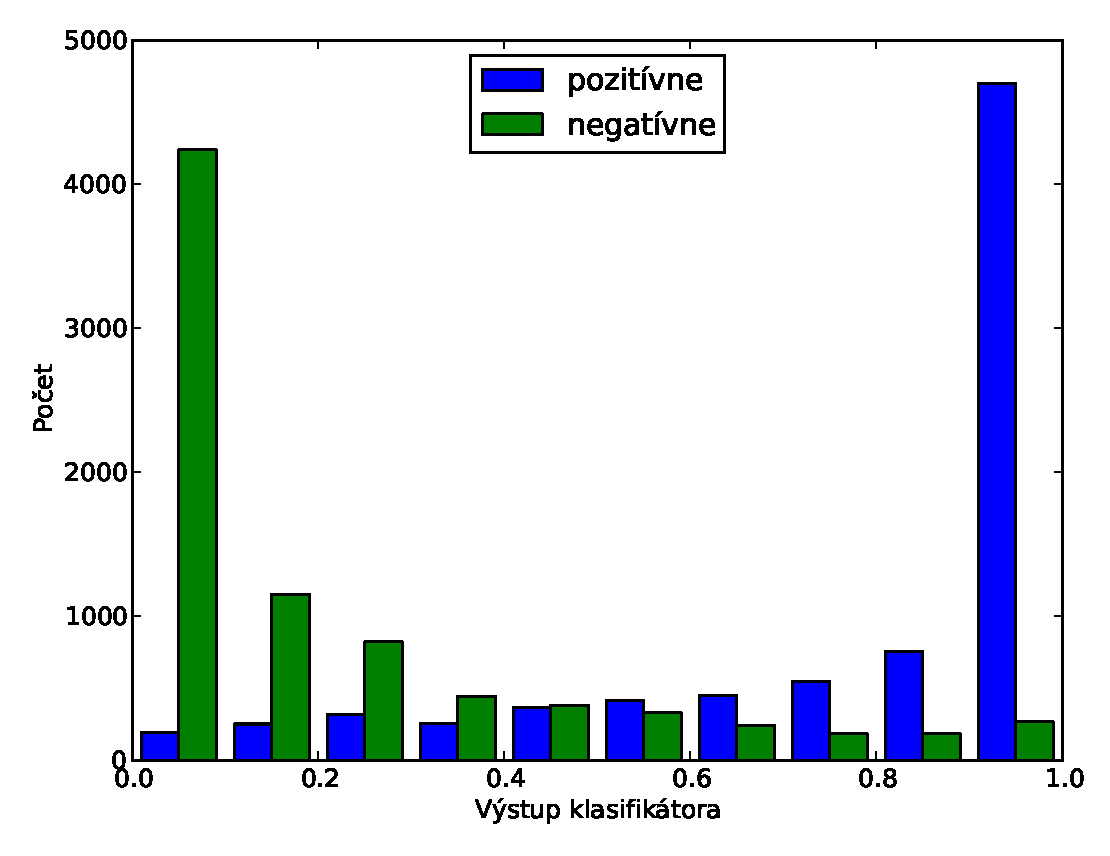
\includegraphics[width=\textwidth]{images/randomforest_combined_5_test}
                \caption{Match klasifikátor}
        \end{subfigure}%
        \qquad %add desired spacing between images, e. g. ~, \quad, \qquad etc.
          %(or a blank line to force the subfigure onto a new line)
        \begin{subfigure}[b]{0.45\textwidth}
                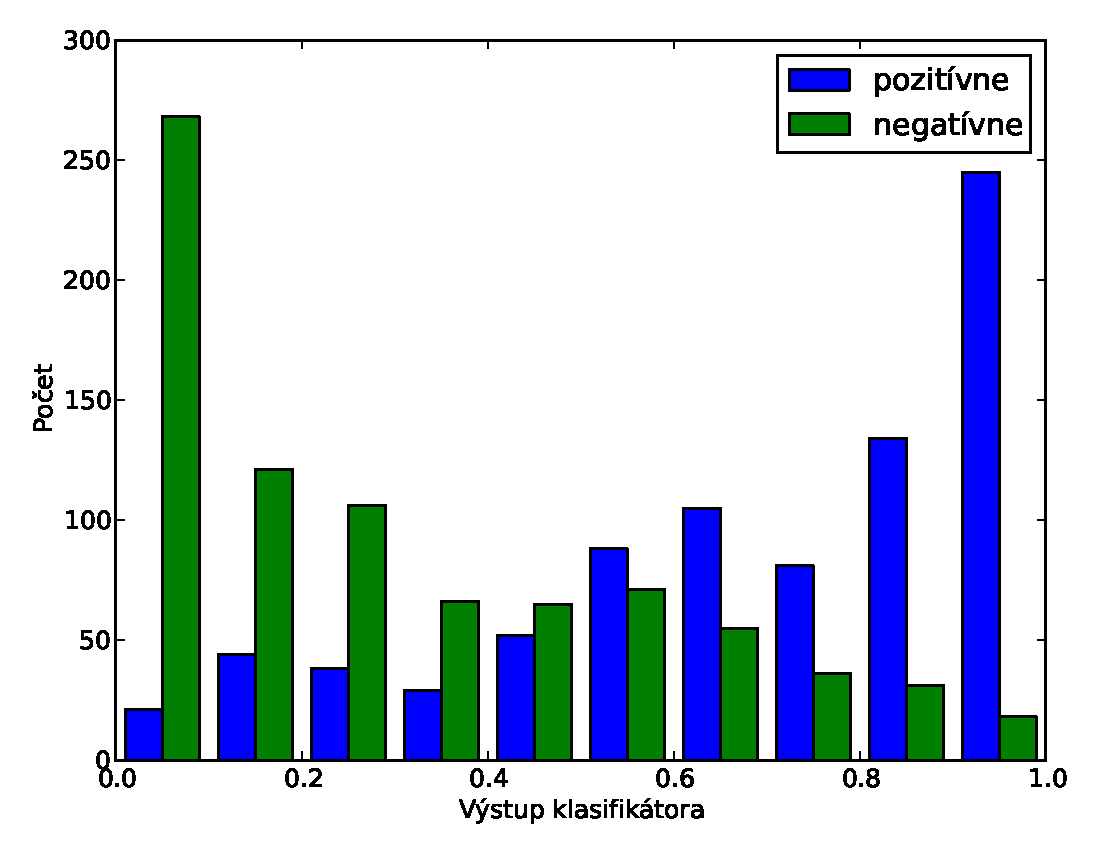
\includegraphics[width=\textwidth]{images/randomforest_combined_5_indel_test}
                \caption{InDel klasifikátor}
        \end{subfigure}
        \caption{Distribúcia výstupu klasifikátora pre pozitívne a negatívne príklady.}
\end{figure}
\end{frame}


\begin{frame}{Dôležitosť atribútov}
\begin{figure}[h]
        \centering
        \begin{subfigure}[b]{0.45\textwidth}
                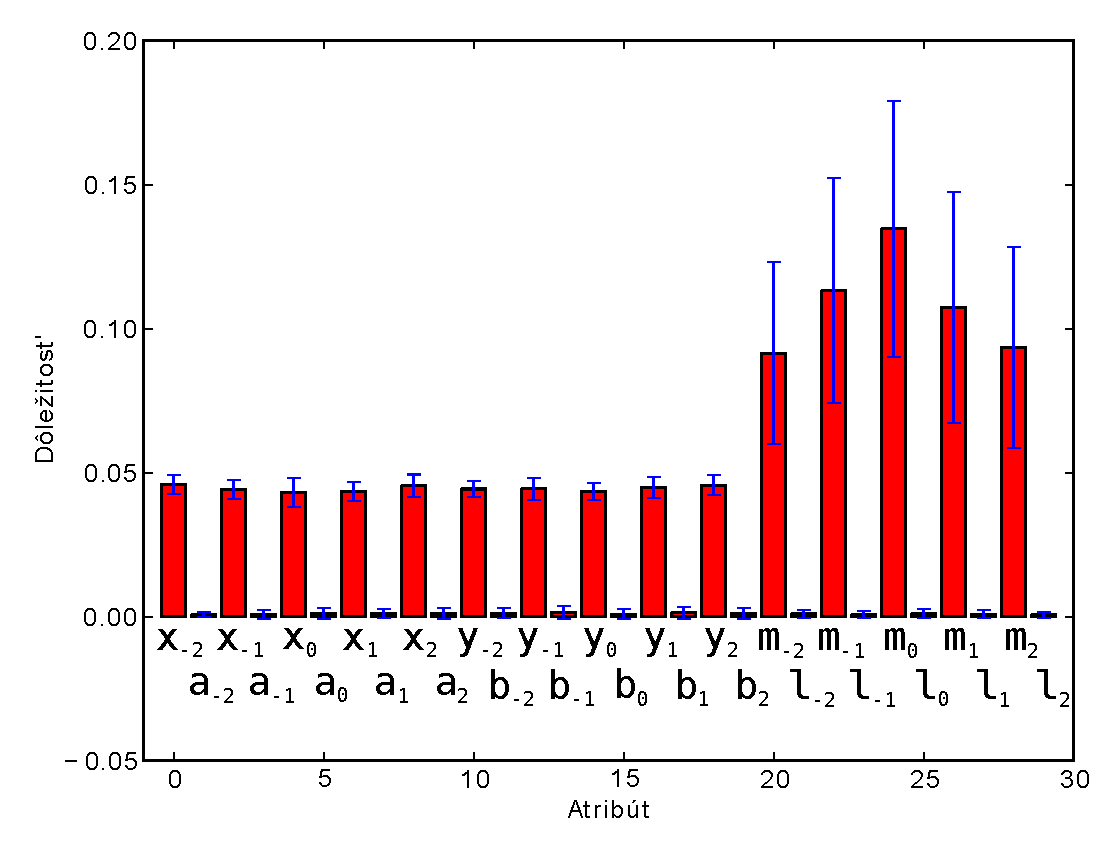
\includegraphics[width=\textwidth]{images/randomforest_combined_5_bars}
                \caption{Match klasifikátor}
        \end{subfigure}%
        \qquad %add desired spacing between images, e. g. ~, \quad, \qquad etc.
          %(or a blank line to force the subfigure onto a new line)
        \begin{subfigure}[b]{0.45\textwidth}
                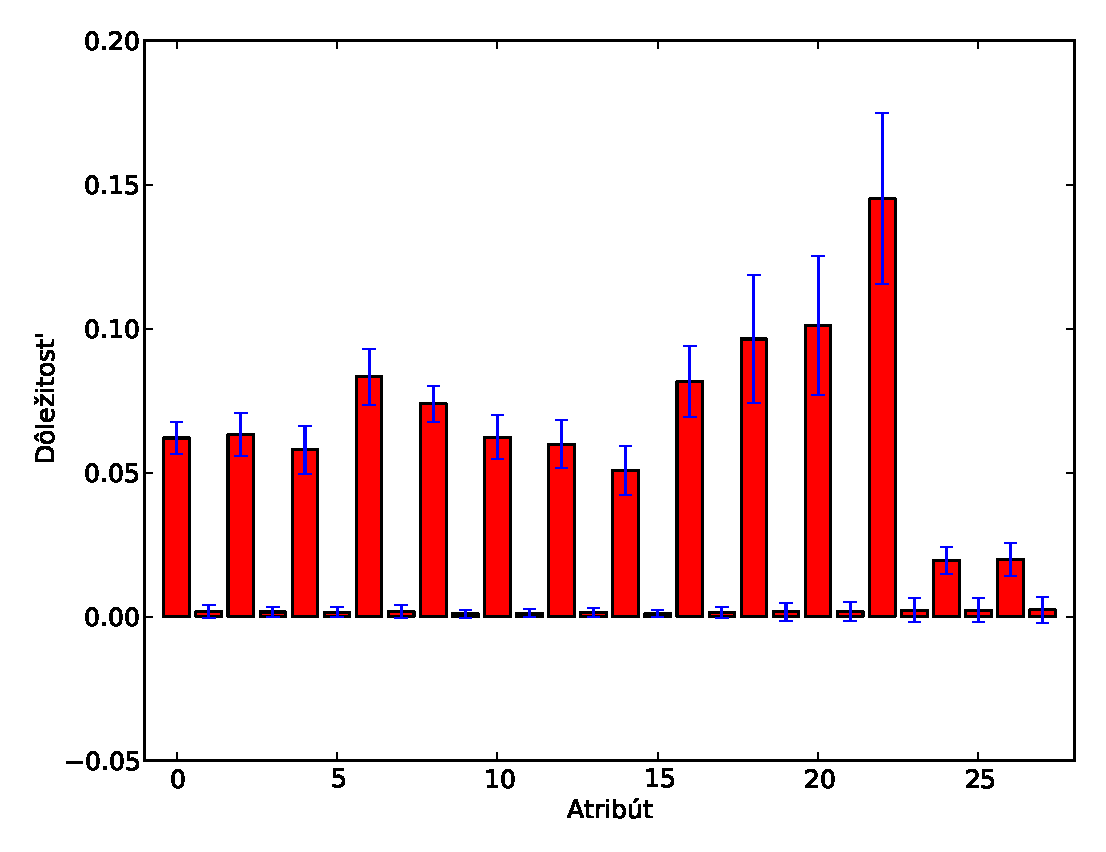
\includegraphics[width=\textwidth]{images/randomforest_combined_5_indel_bars}
                \caption{InDel klasifikátor}
        \end{subfigure}
        \caption{Dôležitosť atribútov v~klasifikátore.}
\end{figure}
\end{frame}

\subsection{Zakomponovanie výsledkov klasifikácie do pHMM}
\begin{frame}{Zakomponovanie výsledkov klasifikácie do pHMM}

\begin{itemize}
  \item skonštruovali sme dva modely pre zarovnanie sekvencií s~anotáciami za pomoci klasifikátora
  \begin{enumerate}
    \item Model s~klasifikátorom ako emisiou
    \item Model s~klasifikátorovou páskou
  \end{enumerate}
  \item založené na párových skrytých Markovovských modeloch.
\end{itemize}

\end{frame}

\begin{frame}{Model s klasifikátorom ako emisiou (Model A)}
  \mbox{}\hfill\raisebox{-\height}[0pt][0pt]{
   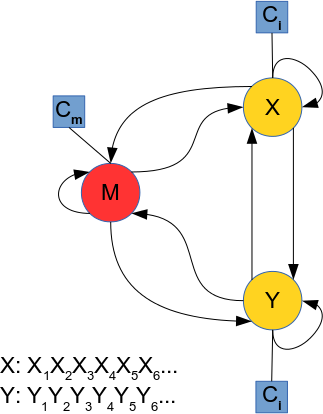
\includegraphics[width=.30\textwidth]{images/zakladny_model}
   }
  \vspace*{-\baselineskip}

  \begin{itemize}
    \item \lenitem{emisné tabuľky stavov nahradíme výstupom z~klasifikátora}
    \item \lenitem{model nie je korektný pravdepodobnostný model, pretože pravdepodobnosti emisií nesčitujú do~1}
    \item \lenitem{prechodové pravdepodobnosti sme natrénovali zo zarovnaní z~trénovacej vzorky}
  \end{itemize}
\end{frame}

% \begin{frame}{Distribúcia výstupu z~klasifikátora}{Match stav}
% \begin{figure}[hbtp]
%     \centering
%     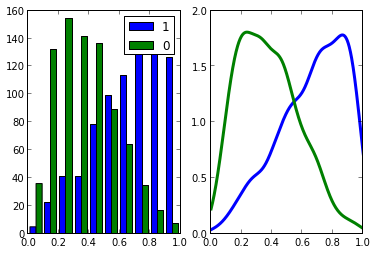
\includegraphics[height=0.5\textheight]{images/clf_m_test.png}
%     \caption{Distribúcia výstupu klasifikátora pre zarovnané (modrá) a nezarovnané (zelená) pozície. Klasifikátor pre match stav s~anotáciou a oknom veľkosti 5 (testovacia množina)}
% \end{figure}
% \end{frame}

% \begin{frame}{Distribúcia výstupu z~klasifikátora}{Insert stav}
% \begin{figure}[hbtp]
%     \centering
%     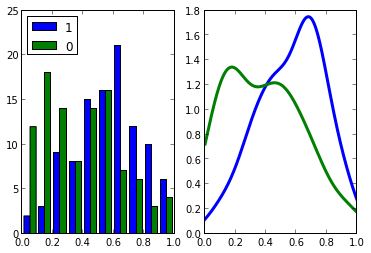
\includegraphics[height=0.5\textheight]{images/clf_i_test.png}
%     \caption{Distribúcia výstupu klasifikátora pre zarovnané pozície (zelená) a pozície zarovnané k~medzere (modrá). Klasifikátor pre insert stav s~anotáciou a oknom veľkosti 5 (testovacia množina)}
% \end{figure}
% \end{frame}


%ToDo: Obrázok
\begin{frame}{Model s~klasifikátorovou páskou (Model B)}
  \mbox{}\hfill\raisebox{-\height}[0pt][0pt]{
   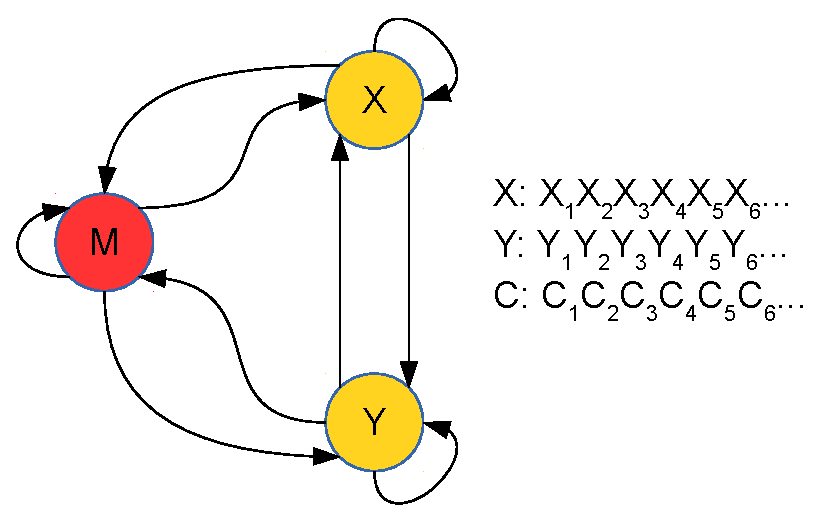
\includegraphics[width=.30\textwidth]{images/model_clf_paska}
   }
  \vspace*{-\baselineskip}

  \begin{itemize}
      \item \lenitem{modelujeme navyše sekvenciu výstupov klasifikátora vo forme pásky}
      \item \lenitem{trénujeme všetky parametre na trénovacej vzorke zarovnaní obohatenej o~pásku s~výstupmi z~klasifikátora}
  \end{itemize}

  \begin{itemize}
    \item \lenitem{páska je cesta v~2D tabuľke výstupov klasifikátorov}
    \item \lenitem{zhoduje sa s~cestou zarovnania}
    \item ak sa pohneme horizontálne, alebo vertikálne, používame Indel klasifikátor a ak sa pohneme diagonálne, tak použijeme Match klasifikátor
  \end{itemize}
\end{frame}

\begin{frame}[fragile]
\begin{figure}[htp]
    \centering
    \begin{subfigure}[m]{0.5\textwidth}
    \centering
    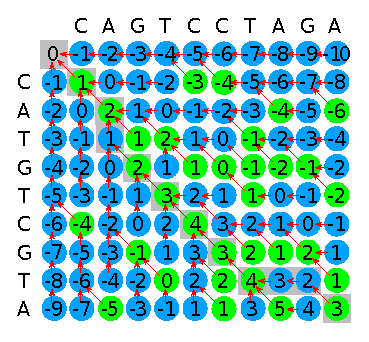
\includegraphics[width=\textwidth]{images/clf_tape}
    \end{subfigure}
    ~
    \begin{subfigure}[m]{0.3\textwidth}
    \centering
    \begin{BVerbatim}[commandchars=\\\{\}]
    CATGTCAT--A
    CA-GTCCTAGA
    {\color{green}MM}{\color{blue}I}{\color{green}MMMMM}{\color{blue}II}{\color{green}M}
    \end{BVerbatim}
    \end{subfigure}
    \caption{Použité klasifikátory v~klasifikátorovej páske}
    \label{fig:clf-tape}
\end{figure}
\end{frame}

% \begin{frame}{Distribúcia výstupu z~klasifikátora}{Match stav - AA}
% \begin{figure}[hbtp]
%     \centering
%     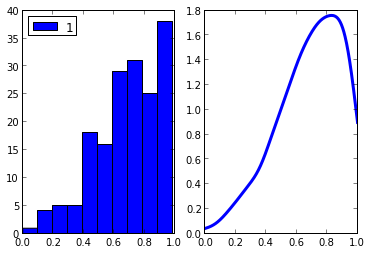
\includegraphics[height=0.55\textheight]{images/distr_aa.png}
%     \caption{Distribúcia výstupu klasifikátora pre match stav v~prípade báz AA zarovnaných k~sebe. Klasifikátor s~anotáciou a oknom veľkosti 5 (testovacia množina)}
% \end{figure}
% \end{frame}

% \begin{frame}{Distribúcia výstupu z~klasifikátora}{Match stav - AC}
% \begin{figure}[hbtp]
%     \centering
%     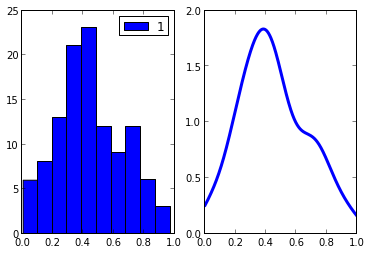
\includegraphics[height=0.55\textheight]{images/distr_ac.png}
%     \caption{Distribúcia výstupu klasifikátora pre match stav v~prípade báz AC zarovnaných k~sebe. Klasifikátor s~anotáciou a oknom veľkosti 5 (testovacia množina)}
% \end{figure}
% \end{frame}

%ToDo: Obrázok
% \begin{frame}{Kombinovaný model}
%   \begin{itemize}
%     \item 3 stavový HMM
%     \begin{itemize}
%       \item Match
%       \item Insert X
%       \item Insert Y
%     \end{itemize}
%     \pause
%     \item Viterbiho algoritmus
%     \begin{itemize}
%     \item pravdepodobnosti získané z natrénovaného klasifikátora
%   \end{itemize}
%   \pause
%   \item rozšírenie sekvencií o anotácie
%   \end{itemize}
% \end{frame}


% \begin{frame}{CRF}
%   \begin{itemize}
%     \item 3 stavový HMM
%     \begin{itemize}
%       \item Match
%       \item Insert X
%       \item Insert Y
%     \end{itemize}
%     \pause
%     \item Viterbiho algoritmus
%     \begin{itemize}
%     \item pravdepodobnosti získané z natrénovaného klasifikátora
%   \end{itemize}
%   \pause
%   \item rozšírenie sekvencií o anotácie
%   \end{itemize}
% \end{frame}

% \subsection{Klasifikátor}
% \begin{frame}{Klasifikátor}
% Random Forest
%   \begin{itemize}
%     \item Zložený z klasifikačných (rozhodovacích) stromov
%     \item Stromy hlasujú o výsledku
%   \end{itemize}
%   \vspace{.5cm}
%   \begin{center}
%   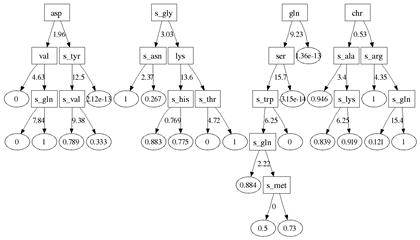
\includegraphics[width=.5\textwidth]{images/random_forest_thumb.png}
%   \end{center}
% \end{frame}


\section{Výsledky}
% \subsection{Metódy vyhodnocovania}
% \begin{frame}{Metódy vyhodnocovania}{Kontrola tranzitivity}
% Ako základnú mieru úspešnosti nášho algoritmu budeme brať kontorlu tranzitivity
%   \begin{itemize}
%     \item Použijeme 3 párové zarovnania 3 sekvencií (každá s~každou)
%     \item Spojíme prvé 2 zarovnania do nového zarovnania
%     \item Porovnáme percentuálne zhody nového s~tretím zarovnaním
%   \end{itemize}
%   % TODO obrazok
% \end{frame}


% \begin{frame}{Dodatočné informácie}
% \begin{figure}[hbtp]
%     \centering
%     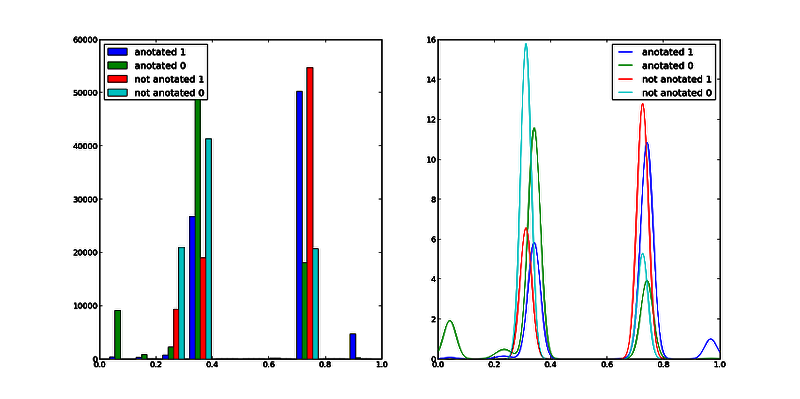
\includegraphics[width=\textwidth]{images/porovnanie_s1w1testset.png}
%     \caption{Porovnanie distribúcie pravdepodobností bez anotácie a s anotáciou (100000 báz, okno veľkosti 1, testovacia množina)}
%     \label{fig:porovnanie_s1w1testset.png}
% \end{figure}
% \end{frame}

% \begin{frame}{Väčšie okno}
%   \begin{itemize}
%     \item Väčšie okno sa prejaví vo väčšom množstve \textit{vlastností}, čo
%     \item Pri malom množstve doplnkovej informácie má výrazný vplyv
%     \item Pri väčšom množstve doplnkovej informácie ich znásobuje
%   \end{itemize}
% \end{frame}

% \begin{frame}{Väčšie okno}
% \begin{figure}[hbtp]
%     \centering
%     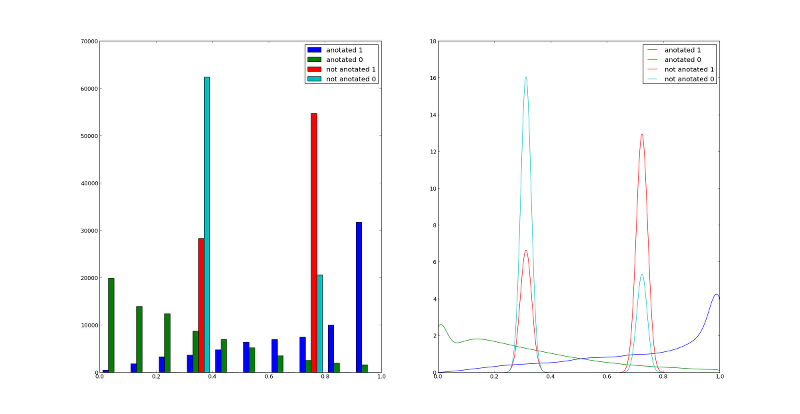
\includegraphics[width=0.9\textwidth]{images/porovnanie_s1w5vsw1testset.png}
%     \caption{Porovnanie distribúcie pravdepodobností bez anotácie a oknom veľkosti 1 a s anotáciou s oknom veľkosti 5 (100000 báz, testovacia množina)}
%     \caption{s1w5vsw1testset}
%     \label{fig:porovnanie_s1w5vsw1testset.png}
% \end{figure}
% \end{frame}



\begin{frame}{Výsledky}

\begin{table}[htp]
\footnotesize
% \catcode`\-=12
\centering
\begin{tabu} to \textwidth {X[l]X[c]X[c]X[c]X[c]X[c]X[c]X[c]X[c]}
\toprule
\multirow{2}{*}{Dáta} &
\multicolumn{2}{c}{Model A} &
\multicolumn{2}{c}{Model B } &
\multicolumn{2}{c}{Ref. Model } &
\multicolumn{2}{c}{Muscle} \\
\cmidrule(r){2-3}\cmidrule(lr){4-5}\cmidrule(lr){6-7}\cmidrule(l){8-9}
& Zhoda & Tranz. & Zhoda & Tranz. & Zhoda & Tranz. & Zhoda & Tranz.\\
\midrule
sim1 & 79,75\% & 44,97\% & 84,35\% & 56,5\% & \textbf{85,78\%} & \textbf{61,03\%} & 82,72\%& 58,76\%\\
sim2 & 70,14\% & --- & \textbf{71,47}\% & --- & 60,38\% & --- & 61,47\% & --- \\
bio & \textbf{91,40\%} & 96,63\% & 91,24\% & \textbf{96,89\%} & 91,34\% & 96,45\% & 91,28\% & 95,98\%\\
\bottomrule
\end{tabu}
\caption[Porovnanie s~existujúcimi zarovnávačmi]{Porovnanie našich modelov s~referenčným modelom a zarovnávačom muscle.}
\label{tab:success-compare}
\end{table}
\begin{itemize}
    \item Tranzitivitu počítame z troch zarovnaní $AB, BC$ a $AC$ ako percentuálnu zhodu medzi zložením prvých dvoch zarovnaní ($AB \circ BC$) a tretieho zarovnania $AC$.
\end{itemize}
\end{frame}



% \begin{frame}{Výsledky}
% \begin{table}[htp]
% \footnotesize
% % \catcode`\-=12
% \centering
% \begin{tabu} to \textwidth {X[l]X[c]X[c]X[c]X[c]X[c]X[c]X[c]X[c]}
% \toprule
% \multirow{2}{*}{Dáta} &
% \multicolumn{2}{c}{Model A} &
% \multicolumn{2}{c}{Model B } &
% \multicolumn{2}{c}{Ref. Model } &
% \multicolumn{2}{c}{Muscle} \\
% \cmidrule(r){2-3}\cmidrule(lr){4-5}\cmidrule(lr){6-7}\cmidrule(l){8-9}
% & Zhoda & Tranz. & Zhoda & Tranz. & Zhoda & Tranz. & Zhoda & Tranz.\\
% \midrule
% sim1 & 20,25\% & 55,03\% & 15,65\% & 43,5\% & \textbf{14,22\%} & \textbf{38,97\%} & 17,28\%& 41,24\%\\
% sim2 & 29,86\% & --- & \textbf{28,53}\% & --- & 39,62\% & --- & 38,53\% & --- \\
% bio & \textbf{8,6\%} & 3,37\% & 8,76\% & \textbf{3,11\%} & 8,66\% & 3,55\% & 8,72\% & 4,02\%\\
% \bottomrule
% \end{tabu}
% \caption{Porovnanie \textit{chyby} našich modelov s~referenčným modelom a zarovnávačom muscle.}
% \label{tab:success-compare}
% \end{table}
% \end{frame}

\section{}
% \begin{frame}{Najbližšie plány}
%   \begin{itemize}
%     \item Dorobiť ostatné modely
%     \item Urobiť experimenty na reálnych dátach
%     \item Experimenty s~deravým oknom, poprípade iné
%     \item V~prvom modeli CRF namiesto HMM?
%   \end{itemize}
% \end{frame}

\begin{frame}[plain, c]
  \transdissolve[duration=5]
  \begin{center}
  \textbf{\color{Green} \LARGE Ďakujem za pozornosť!}

  \vspace{1cm}

  
\includegraphics[width=.30\textwidth]{images/realigner}

  \vspace{.5cm}

  \url{https://github.com/mhozza/realigner}
  \end{center}


\end{frame}

\begin{frame}[allowframebreaks]{Literatúra}
  \bibliographystyle{apalike}
  \bibliography{references}
\end{frame}


\end{document}
